\section{Conclusions}

\subsection{Particle entanglement of one-dimensional spinless fermions}

The empirical scaling form for the one-particle entanglement entropy in the $t-V$ model proposed in \cite{Zozulya:2008kb} was confirmed analytically. This scaling suggested that the one-particle entanglement entropy should go as $S(n,N) = \ln{{N}\choose{n}} + a + \mathcal{O}(\frac{1}{N^{\gamma}})$, where $n$ is the number of particles in the subsystem, $N$ is the total number of particles in the system, and $a$ and $\gamma$ are parameters that depend on the interaction between the fermions and hence the Luttinger Parameter, $K$.  The first term on the scaling form is the free-fermion contribution to the entanglement entropy. Having confirmed analytically the empirically proposed scaling of the one-particle entanglement entropy, the entanglement contribution coming from particle interactions was calculated. To calculate the particle interaction contribution to the one-particle entanglement entropy,  $S(n,N) - \ln{{N}\choose{n}}$ was calculated at various values of particle interaction strengths $V/t$. Not only agreement was again seen between numerical results, Tomonaga-Luttinger Liquid (TLL) theory and the proposed scaling, but it was also seen that the one-particle entropy was sensitive to phase transitions in the $t-V$ model.

\subsection{Accessible spatial entanglement entropy of one-dimensional spinless fermions}

The amount of spatial entanglement in the $t-V$ model that is accessible as a resource was computed analytically and via exact diagonalization as a function of interaction strength. It was seen that this type of entanglement was also sensitive to the phase transitions of the model. At the continuous phase transition, a peak was observed and a power-law scaling suggests that in the limit of inifitely many fermions, this peak would move exactly to the value of the phase transition. The difference between the full and the accessible entanglement entropies was also computed. Also via exact diagonalization, it was confirmed that the probabilities of measuring a number $n$ of particles are Gaussianly distributed.

\subsection{Summary}

This work confirmed the effectiveness of quantum entanglement as a probe for quantum phase transitions. The theoretical knowledge gained from this is very rich on its own, but it will also be of experimental value in the near future. The advent of quantum computers, and other quantum technologies, has brought the need to build devices that have to be cooled to near zero Kelvin temperatures, for example the qubits in a quantum computer. At zero temperature, phase transitions are driven by purely quantum mechanical effects. Then, having ways of probing the phase of the quantum device will be necessary to understand its microscopical physical properties, and therefore the macroscopic ones too.

It was also seen that the way a system is partitioned will give different insights about the entanglement of a system. Partitioning a system into spatial subregions gives insights about how information is shared across the boundary between the regions. On the other hand, a particle partition gives a length-scale free and particle-statistics dependent idea of how information is shared between entangled groups of particles. Although the entanglement under both of these types of partitions was used to successfully detect phase transitions in the $t-V$ model, features were seen using one type of entanglement that were not seen with the other. For example, for particle entanglement, it was seen how the von Neumann and R\'enyi entropies had a contribution due to not only particle interactions but also the antisymmetrization of the wave function due to fermionic statistics. Under a spatial bipartition, the entanglement exhibits a peak at the continuous phase transition that scales with system size towards the phase transition. More examples can be pin pointed of properties that were seen under each type of partition, but the bottom line is that different features will be seen for each. Thus, it will be of benefit moving forward to consider not only one, but both types of partitions when studying entanglement, to give a broader understanding of the particular physical system under study.

Superselection rules have the effect of reducing the amount of entanglement that can be used as a resource. Recall that one of the main goals for the study of entanglement is to build real life devices that rely on this phenomenon to function, such as a quantum computer. The von Neumann and R\'enyi entropies are good enough to pick up interesting features of the system, like phase transitions. But to actually use the entanglement as a resource, superselection rules that restrict the number of states that can be prepared must be accounted for. By considering the particle number superselection rule, it was seen that the amount of entanglement accessible as a resource is always less or equal to the von Neumann and R\'enyi entropy. The calculation of the accessible entanglement should be more ubiquitous in the theoretical study of entangled systems, since it gives a measure that more closely approximates the entanglement that may be measured in an experimental setting.


\section{Future work}

	In this section, future projects are discussed. Some of these projects stem from unanswered questions in previous work, while some of them will be completely new.
	
	\subsection{Power law scaling of entanglement peak in the $tV$ model}
	
	%%%%%%%%%%
	\begin{figure}[h]
	\begin{center}
	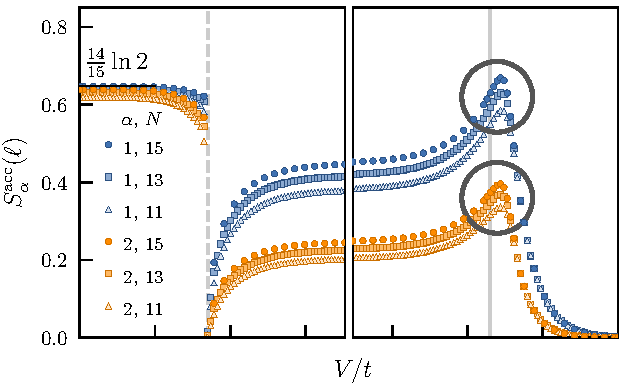
\includegraphics[scale=1.0]{operationalEntanglementEntropies_SOP5_withPeakCircles.pdf}
	\end{center}
	\caption{Accessible entanglement entropies as a function of interaction strength in the $t-V$ model. The circles enclose a region where both the von Neumann and R\'enyi entanglement entropies attain a maximum value. As the total number of particles $N$ increases, this maximum seems to be shifting to the left, closer to the phase transition $V/t=2$.}
	\label{fig:OEE_circledPeaks}
	\end{figure}
	%%%%%%%%%%
	
	In the $t-V$ model, there are two known phase transitions, a first order one at $V/t=-2$, and a continuous one at $V/t=2$. From Figure \ref{fig:OEE_circledPeaks}, it can be seen that the accessible entanglement entropies are sensitive to both types of transition. Interestingly, this sensitivity to the transition in $V/t=2$ expresses itself as a peak of entanglement. Moreover, the interaction strength at which this peak of entanglement occurs moves closer to the exact value of the continuous phase transition as the number of particles in the system increases.  
	
	%%%%%%%%%%
	\begin{figure}[h!]
	\begin{center}
	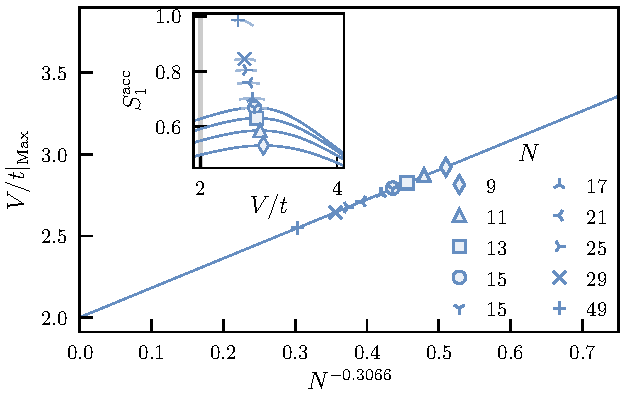
\includegraphics[scale=1.0]{peakScalingOddN.pdf}
	\end{center}
	\caption{Interaction strength at which the maximum $S_{1}^{\mathrm{acc}}$ occurs as a 	function of the total number of particles $N$. The exponent of $N$ was obtained from a l	inear fitting of $\ln N$ vs. $\ln{(V/t - 2)}$.  Although very few points are plotted due to 	memory limitations, they agree with the hypothesis that for $N \to \infty$, the peak of 	von Neumann accessible entanglement occurs at the phase transition $V/t = 2$. Inset: 	$S_{1}^{\mathrm{acc}}$ as a function of interaction strength $V/t$ for various $N$ 		around the neighborhood of the peak.}
	\label{fig:peakScalingOddN}
	\end{figure}
	%%%%%%%%%%
	
	Figure \ref{fig:peakScalingOddN} shows the value where the entanglement peak occurs for various system sizes. The fact that all the points lie on a line that intercepts the vertical axis at $V/t_{Max}=2$ is very promising. Nevertheless, the current scaling exponent of $-0.2545$ should not be taken for granted due to how small the systems currently are. Indeed, the continuous phase transition should occur in the $t-V$ model at $V/t=2$, but this is for a system where $N \to \infty$. More data points, corresponding to large systems are still be needed to get closer to this intercept and confirm the power law scaling. To aid in reaching this larger system sizes, Density Matrix Renormalization Group (DMRG) will be employed \cite{SCHOLLWOCK201196, itensor}. With DMRG, it is expected that systems consisting of roughly 100 particles can be simulated.

	
	\subsection{Filling fraction dependence of entanglement}
	
	The $t-V$ model results presented in this thesis were focused on the special case of half-filling. That is, only half of the lattice sites were had particles in them ($N = L/2$). For this case, the exact results for the phase transitions are mapped from the XXZ spin-$1/2$ model. For other filling fractions, a theory has yet to be developed. Figure \ref{fig:fillingFractionDependence} shows the accessible entanglement entropies for various filling fractions ranging from $1/14$ to $1/2$. Expanding the results outside the realm of half filling will help to learn if some of the interesting features observed, such as the scaling of the accessible entanglement peak and the Gaussian distribution of local particle number probabilities in the TLL phase, are independent of filling fraction. 
	
	%Figure 8
	%%%%%%%%%%
	\begin{figure}[h!]
	\begin{center}
	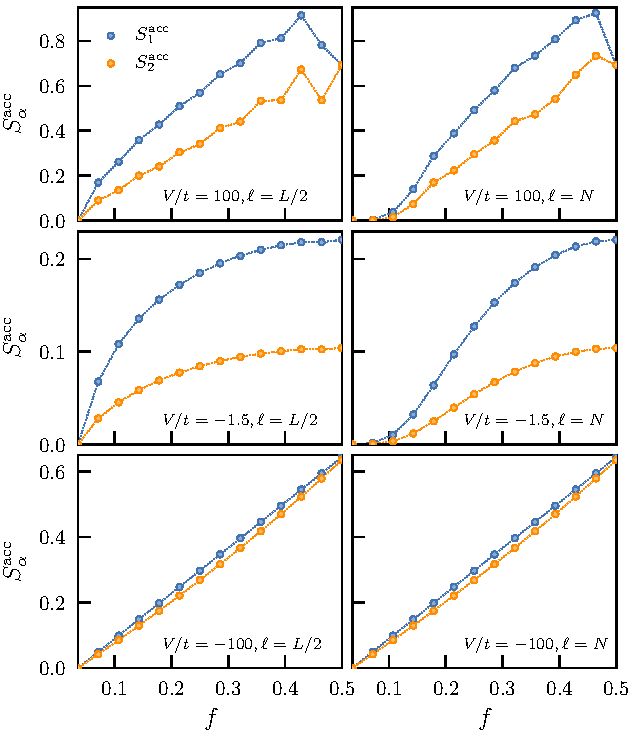
\includegraphics[scale=1.0]{fillingFractionDependence.pdf}
	\end{center}
	\caption{Accessible entanglement entropies $S_{\alpha}^{\mathrm{acc}}(\ell)$ for $		\alpha = 1,2$ as a function of filling fraction $N/L$. The lattice size was kept fixed at 		$L=28$ sites and the total number of particles were $N=1,2,3...14$. For the left column, 	the spatial partition $\ell$ was kept fixed at half the lattice size, $\ell = L/2$. For the right 	column, it was set to equal the total number of particles $N$. The interaction strengths 	$V/t$ are indicated in each of the plots and correspond to values from each of the three 	phases of the $t-V$ model.}
	\label{fig:fillingFractionDependence}
	\end{figure}
	%%%%%%%%%%
	
	\subsection{Accessible entanglement via quantum gates}
	
	The endgame for the study of accessible entanglement entropies is to exploit the entanglement of a system as a resource. Motivated by this, we are currently working on building a quantum circuit that reproduces the accessible entanglement measurement process. After coming up with the appropriate quantum circuit, the results will be tested on IBM's quantum computer \cite{IBM:QM}.
%
	%\cite{IBMQuantumExp:2018:Online}.
	
	\subsection{Entanglement in the Bose-Hubbard model}
	
	Another project in the works is calculating accessible entanglement entropies in the Bose-Hubbard (BH) model. In the study of fermionic systems, such as the $t-V$ model, methods like exact diagonalization and density matrix renormalization group must be used to due to the infamous sign problem. The high memory cost of these methods restricts simulations to only relatively small system sizes and low dimensions. The sign problem does not exist in bosonic models and thus quantum Monte Carlo (QMC) methods can be used. QMC will allow the study of much larger systems than the ones presented here \cite{Hastings:2010dc, Herdman:2016ep}.